\subsection{Neural Network}

Neural Network (NN) is a classifier that tries to replicate the structure of the human thought.

Being the purpose of the paper to compare the performance of SVM vs NN, our second approach was to implement a Neural Network with a Multi-layer Perceptron Classifier \cite{nn-mlp-classifier}.

Just as in our SVM flow, we initially divide our data in two subsets:

\begin{itemize} 
\item Training subset:  \(80\%\)
\item Testing subset:  \(20\%\).
\end{itemize}


Similar to what was done in SVM, we used HOG as our feature extractor. Hence, the specific implementation we used has 3 layers: \(Input Layer \rightarrow Hidden Layer \rightarrow Output Layer\), with the follow specification:

\begin{itemize} 
\item Input Layer: \(128\) neurons (the respective number of features extracted by HOG);
\item Hidden Layer: \(10\) neurons (as default value, the optimized number of neurons will be specified ahead);
\item Output Layer: \(1\) neuron.
\end{itemize}

Furthermore, we used \textit{RELU} as the activation function, the loss function we used was \textit{Log-Loss Function}, using the \textit{LBFGS} weight optimizer (we decide to use \textit{LBFGS}, because, according to Scikit-Learn documentation \cite{nn-mlp-classifier}, it can converge faster and perform better, given smaller datasets, which is our case), and has the default learning rate, we used \( \alpha = 0.001 \), which will be optimized further ahead. To summarize we can see the initial configuration of our Neural Network in table \ref{table:nn-initial-configuration}.

\begin{table}[htbp]
\centering
\caption{NN - Initial Configuration}
\begin{tabular}{ |c|c| } 
 \hline
 \textbf{Train Data} & 80\% \\ 
 \hline
 \textbf{Test Data} & 20\% \\ 
 \hline
 \textbf{Input Layer} & \(128\) neurons \\ 
 \hline
 \textbf{Hidden Layer} & [10, 20, 30, 40, 50, 60, 70] neurons, \(default = 10\) \\ 
 \hline
 \textbf{Output Layer} & \(1\) neuron \\ 
 \hline
 \textbf{Activation Function} & \textit{RELU} \\ 
 \hline
 \textbf{Loss Function} & \textit{Log-Loss Function}, via \textit{LBFGS} weight optimizer \\ 
 \hline
 \textbf{Learning Rate (\(\alpha\))} & [0.001, 0.01, 0.05, 0.1, 0.5, 1, 10], \(default = 0.001\) \\ 
 \hline
 \textbf{Number of Iterations} & [100, 200, 300, ..., 900, 1000], \(default = 100\) \\ 
 \hline
\end{tabular}
\label{table:nn-initial-configuration}
\end{table}

As done in the previous section, the SVM aproach \ref{svm}, we optimized the hyper-parameters of the NN model to enable its best performance. Just like in SVM, we did this by applying K-Fold Cross Validation, with \(K = 5\). The hyper-parameters we decided to vary, and consequently optimize, were as follows:

\begin{itemize} 
\item Hidden Layer size (the number of neurons in the Hidden Layer);
\item Learning rate (\(\alpha\));
\item Number of iterations.
\end{itemize}

After validating every combination, as we can see in figure \ref{fig:nn-cross-validation}, our model performed the best when:

\begin{itemize} 
\item \( HiddenLayerSize = 60 \) neurons;
\item \( \alpha = 1 \);
\item \( NumberOfIterations = 700 \).
\end{itemize}

\begin{figure}[htbp]
\centerline{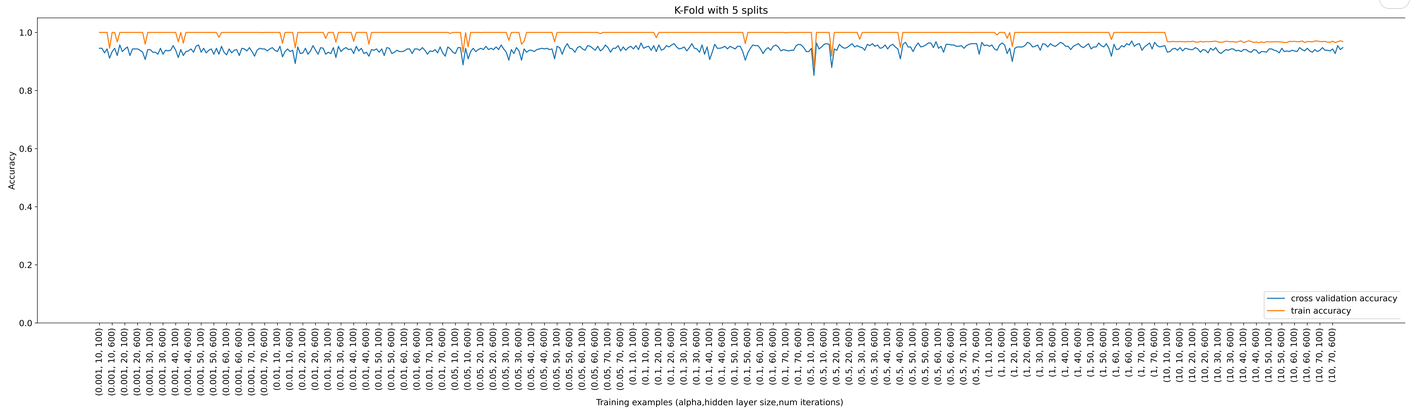
\includegraphics[width=1\linewidth]{images/nn_cross_validation.png}}
\caption{NN - Cross-Validation using multiple-value combinations}
\label{fig:nn-cross-validation}
\end{figure}

Based on the Cross Validation data, we created a Neural Network with a Multi-layer Perceptron Classifier, and a final configuration that can be seen in table \ref{table:nn-final-configuration}.

\begin{table}[htbp]
\centering
\caption{NN - Final Configuration}
\begin{tabular}{ |c|c| } 
 \hline
 \textbf{Train Data} & 80\% \\ 
 \hline
 \textbf{Test Data} & 20\% \\ 
 \hline
 \textbf{Input Layer} & \(128\) neurons \\ 
 \hline
 \textbf{Hidden Layer} & \(60\) neurons \\ 
 \hline
 \textbf{Output Layer} & \(1\) neuron \\ 
 \hline
 \textbf{Activation Function} & \textit{RELU} \\ 
 \hline
 \textbf{Loss Function} & \textit{Log-Loss Function}, via \textit{LBFGS} \\ 
 \hline
 \textbf{Learning Rate (\(\alpha\))} & \(\alpha = 1\) \\ 
 \hline
 \textbf{Number of Iterations} & 700 \\ 
 \hline
\end{tabular}
\label{table:nn-final-configuration}
\end{table}

Finally, and as we did in our SVM approach, to ensure that the model didn't end up in a local minimum, and that our model was actually learning we run the all process 50 times and calculated the mean values to both train and test phases.